\section{\codename}
\label{sec:framework}

% The architecture of \codename is depicted in Figure~\ref{fig:framework}. 
% Beginning with a dataset of Android apps, the first step is to extract pertinent features from these apps.
% These features are then meticulously stored in a feature database. More details are provided in~\ref{sub:feature_db}.
% Subsequently, a dedicated preprocessor is utilized to transform (including retrieving and encoding) these features.
% After that, we proceed to train an ML model and assess its performance in detecting malware.

% % The framework is crafted with two guiding principles at its core: modularization and flexibility.
% \codename is designed with modularity in mind, making it easy to extend and customize.
% This is achieved by decoupling it into three distinct modules: \textit{feature database}, \textit{preprocessor}, and \textit{ML model}.
% Given the structured format of the \textit{feature database}, one can easily incorporate new features and integrate them into the assessment pipeline.
% Moreover, the \textit{preprocessor} can be tailored to accommodate various approaches, granting users the flexibility to determine what/how features are used.
% The \textit{ML model} is preloaded with various ML models, such as SVM, MLP, CNN, and AE.
% Alternatively, \codename also supports custom models, allowing users to incorporate their own models into the framework.

% \begin{figure}[t]
%     \centering
%     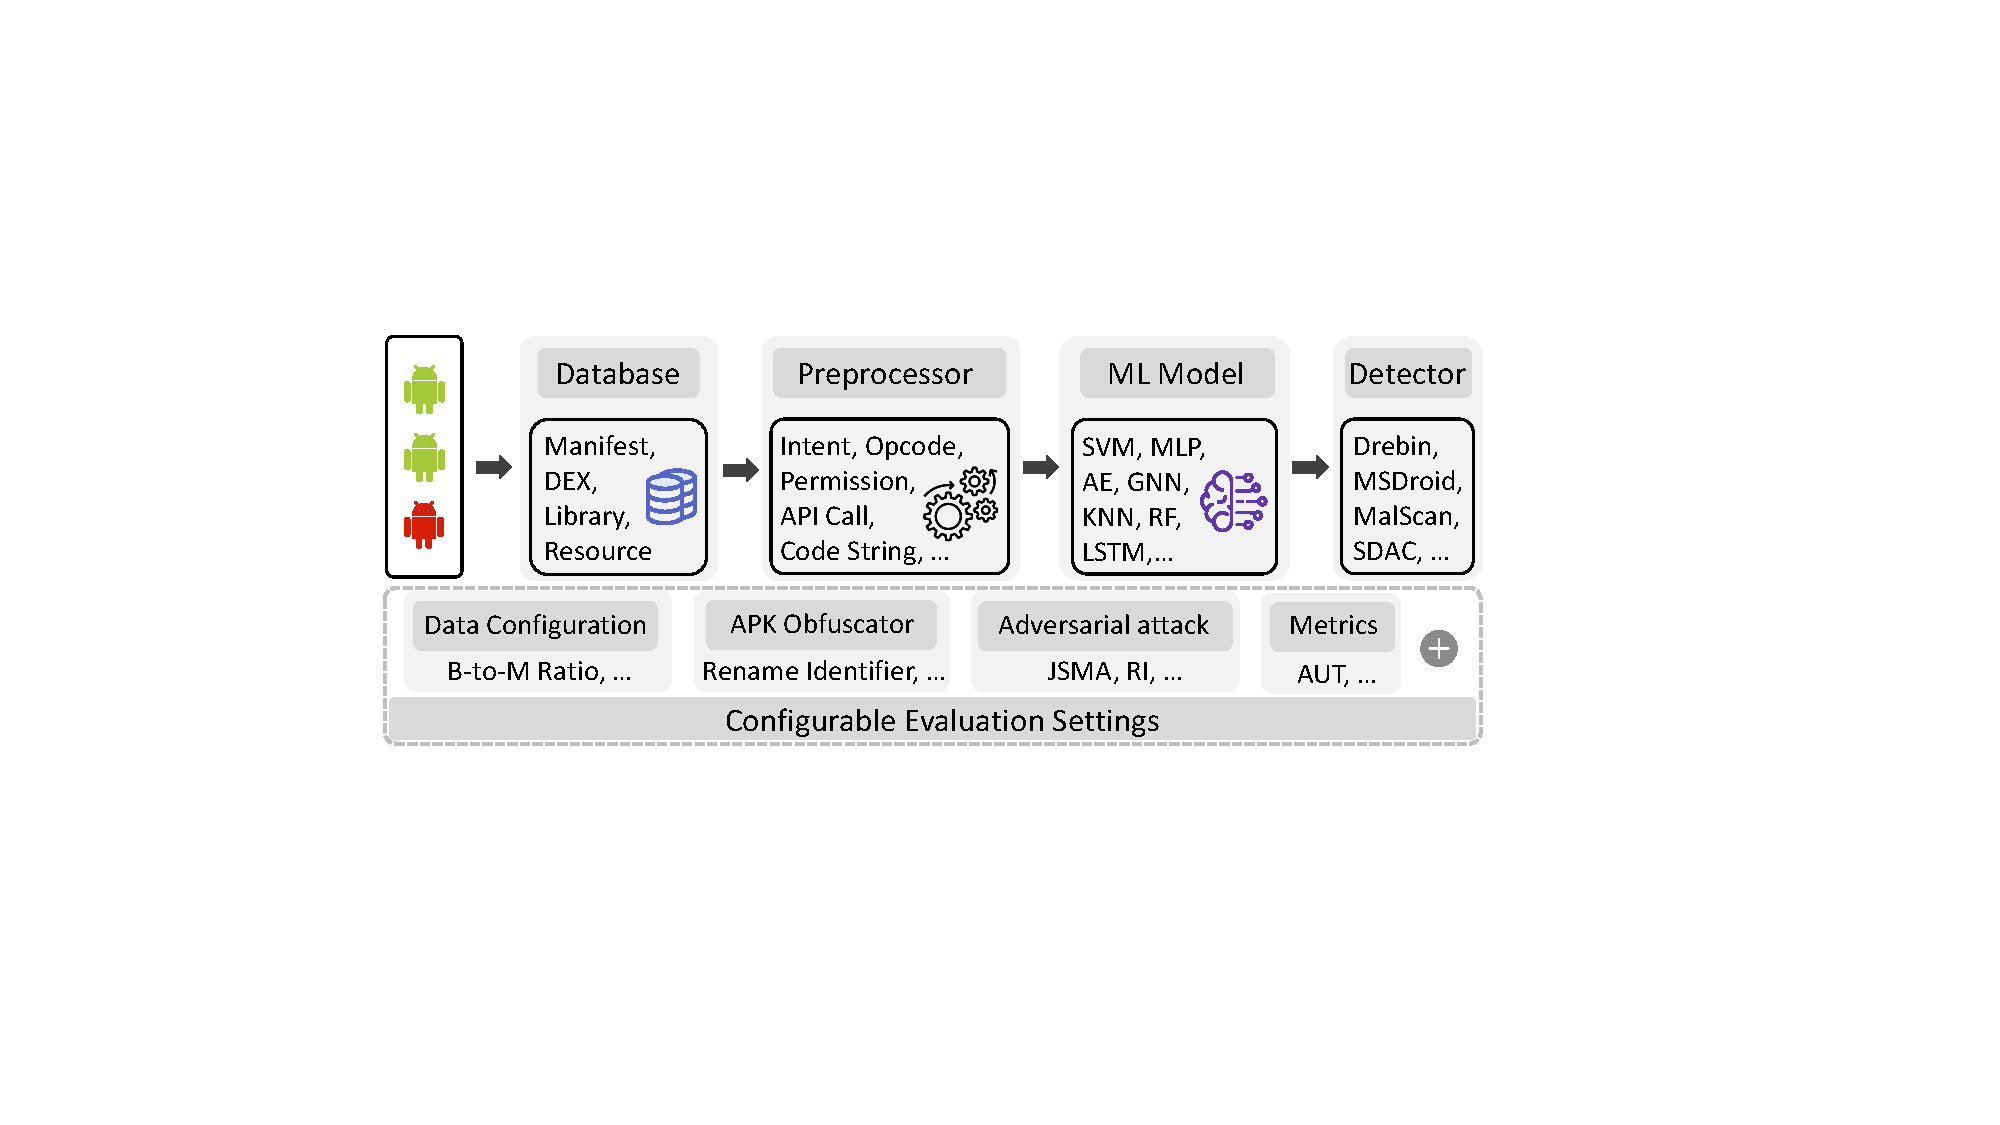
\includegraphics[width=0.94\linewidth]{fig/framework.pdf}
%     \caption{The architecture of \codename.}
%     \label{fig:framework}
%     % \vspace{-0.6cm}
% \end{figure}

% % Following the feature storing format in the {\em feature database}, it is easy to aggregate new features into the framework.
% % With this design, it is easy to design an additional feature extractor and store the derived features in the {\em feature database}, ensuring a smooth integration into the assessment pipeline.
% % Additionally, the {\em preprocessor} can be tailored to accommodate various approaches, granting users the flexibility to choose and adapt feature usage as required.
% \codename also provides a configurable experimental setting to support a wide range of evaluation scenarios.
% Parameters such as the ratio of goodware-to-malware, training data sizes, and time decay are all adjustable.
% This enables users to meticulously select APK samples for diverse evaluation contexts, ensuring comprehensive and accurate assessments.
% Moreover, \codename integrates an APK obfuscator~\cite{aonzo2020obfuscapk}, allowing for obfuscation prior to feature extraction. 
% It also possesses the capability to produce adversarial samples, enabling a robust assessment of model resilience.
% % Leveraging the capabilities of \codename, we re-implement the approaches described in Section~\ref{sec:approach_analysis} and assess them with our curated dataset.
% % We further analyze the evaluation outcomes to provide deeper insights into the current ML-based Android malware detection in Section~\ref{sec:evaluation}.

% % \bulletpoint{Implementation}
% % \codename is developed in 17K lines of Python code.
% % To ensure consistency and mitigate biases from different feature extraction toolchains and learning frameworks, we adopt standardized techniques across all tasks.
% % For feature extraction, we use Androguard to disassemble APK files and derive features such as permissions, intents, and program graphs. 
% % LibRadar helps in identifying third-party libraries within the applications, while Angr is used for analyzing native libraries and capturing essential features like opcodes and API calls. 
% % When it comes to training ML models, the scikit-learn library is our choice for traditional ML algorithms like SVM, KNN, and RF.
% % On the other hand, for DL architectures such as CNN, LSTM, GNN, and AE, we resort to Pytorch.
% % This uniform approach ensures a balanced evaluation, concentrating purely on the uniqueness and performance of each method.
% % Details about the hyper-parameters of these models are provided in Appendix~\ref{sub:hyperparameters}.

\begin{figure}[t]
    \centering
    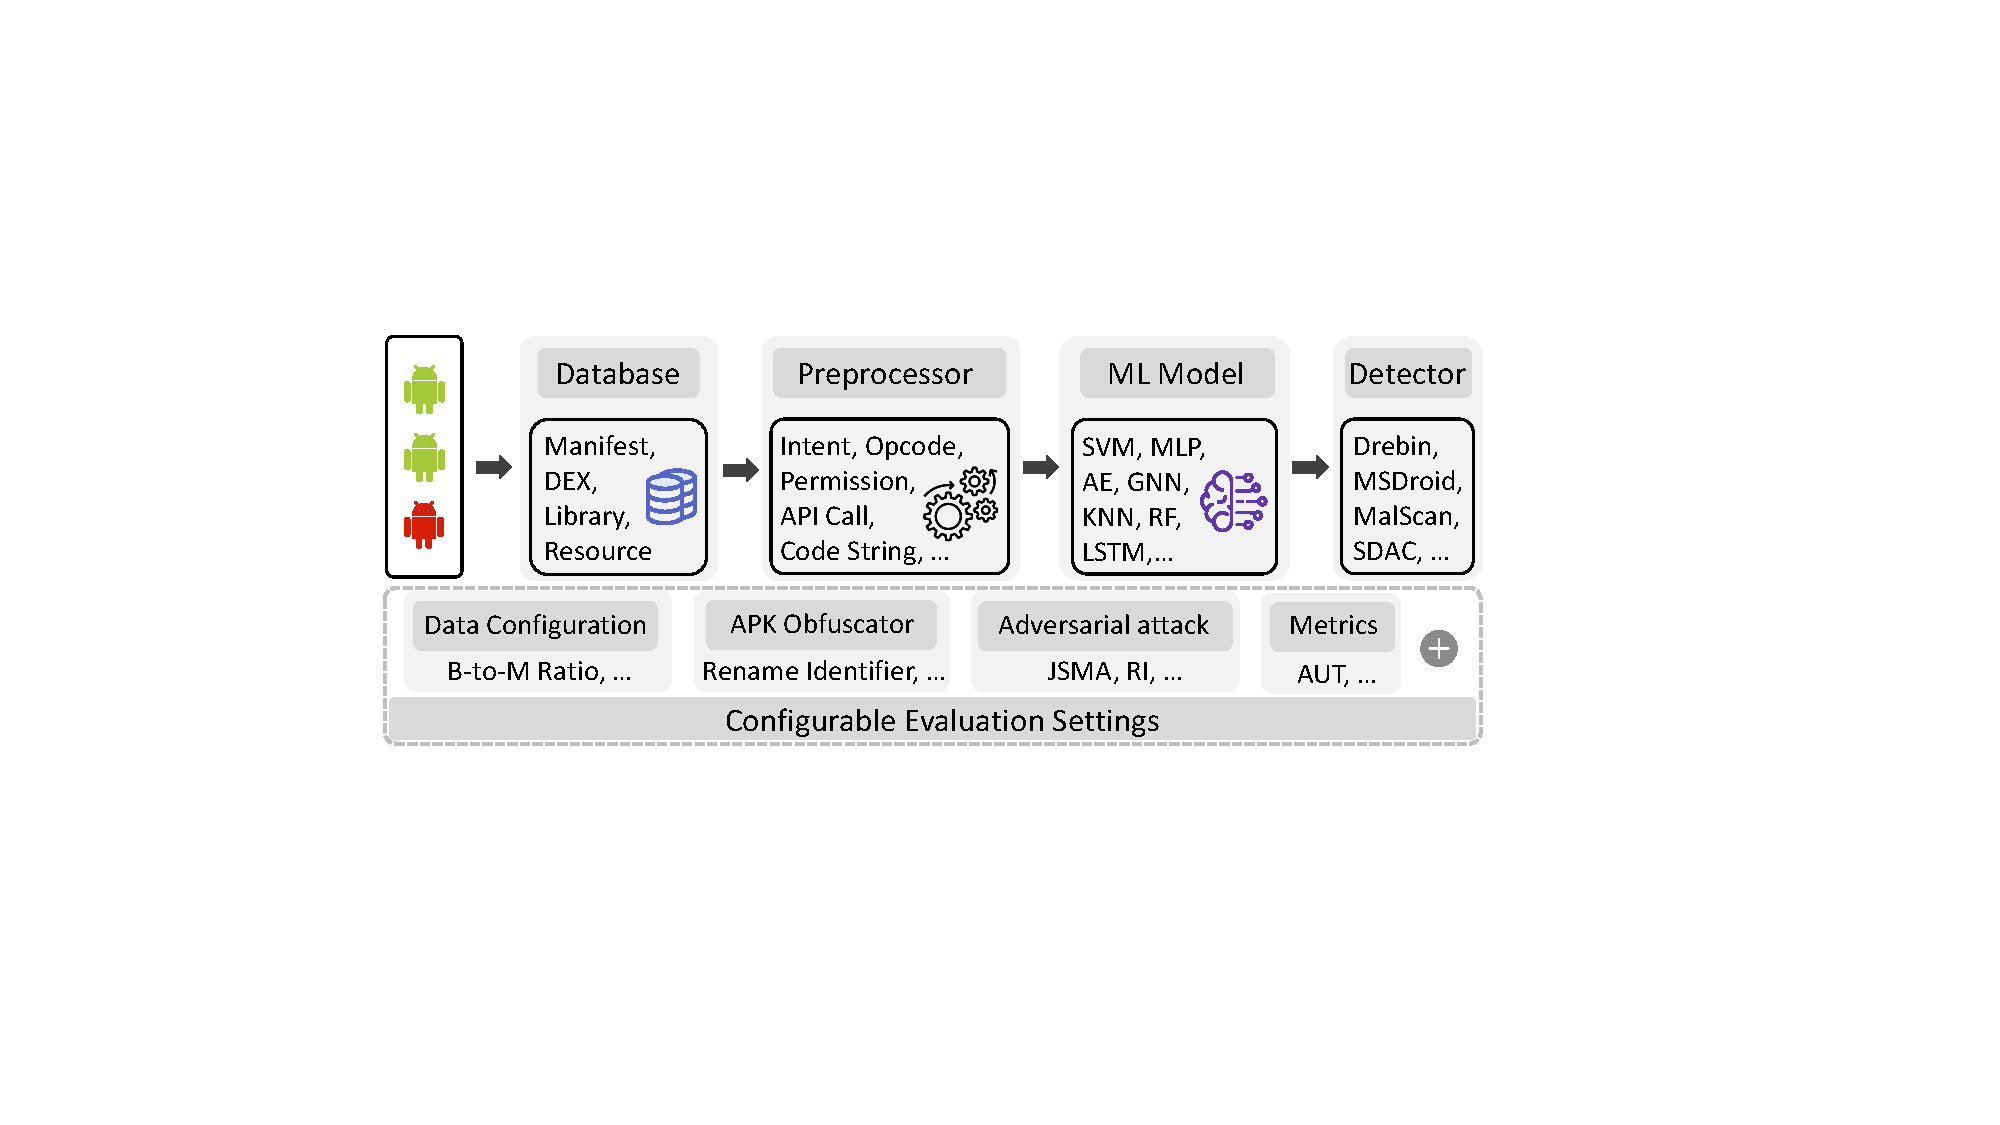
\includegraphics[width=0.74\linewidth]{fig/framework.pdf}
    \vspace{-0.1cm}
    \caption{The architecture of \codename.}
    \label{fig:framework}
    \vspace{-0.3cm}
\end{figure}

% Having analyzed existing ML-based Android malware detection approaches, we propose a general-purpose framework, \codename, to facilitate the development and evaluation of new Android malware detectors.

To support experimental reproducibility and fair comparison, we propose a general-purpose framework, \codename, guided by the detection workflow discussed in Section~\ref{sec:systematic_investigation}, to facilitate the development and evaluation of new Android malware detectors.
Figure~\ref{fig:framework} illustrates the overall architecture and workflow of \codename.
% It starts with a collection of apps, from which a set of features is extracted and stored in a {\em feature database}.
The process begins with a collection of apps, from which a set of features is extracted and stored in a {\em feature database}.
These features are then processed by a {\em preprocessor}, which transformes them into numerical vectors.
A selected {\em ML model} is subsequently trained and evaluated to detect malicious applications.
Furthermore, \codename provides configurable experimental settings to support diverse real-world scenarios, such as varying goodware-to-malware ratios, different training data sizes, and robustness assessments against adversarial attacks.
% It is implemented in 17K lines of Python code, detailed in Appendix~\ref{sub:implementation}.
%
% The framework is crafted with two guiding principles at its core: modularization and flexibility.
% \jh{\codename is modular, which makes it easy to extend and customize according to various requirements.}
% This is achieved by decoupling it into three modules: \textit{feature database}, \textit{preprocessor}, and \textit{ML model}.
% Given the structured format of the \textit{feature database}, one can easily incorporate new features and integrate them into the assessment pipeline.
% Moreover, the \textit{preprocessor} can be tailored to accommodate various approaches, granting users the flexibility to determine what/how features are used.
% The \textit{ML model} is preloaded with various ML models, such as SVM, MLP, CNN, and AE.
% Alternatively, \codename also supports custom models, allowing users to incorporate their own models into the framework.
% Given the structured format of the \textit{feature database} (details can be found in~\ref{sub:feature_db}), one can easily incorporate new features and integrate them into the assessment pipeline.

This modular design of \codename simplifies the development of ML-based Android malware detectors. Three key modules, \textit{feature database}, \textit{preprocessor}, and \textit{ML model}, captures the main aspects of designing ML solutions for Android malware detection.
% \textit{Feature database} organizes the extracted features categorically, including Manifest, ProgramGraph, DisassembledCode, and SharedLibrary, which can be easily extended to incorporate new features.
The \textit{feature database} organizes extracted features categorically according to their sources, as discussed in Section~\ref{sub:apk_characterization}, including Manifest, Dex, Library, and Resource. 
For example, the Manifest category contains features extracted from the AndroidManifest.xml file, such as permissions, intents, and application components.
Further details about the feature database are provided in Appendix~\ref{sub:feature_db}.
Notably, all features are stored in a manner consistent with our APK characterization taxonomy.
Each directory corresponds to a specific feature source, and the features of a given APK are distributed accordingly --- for instance, Hardware Components and Application Components under Manifest; API Calls, Opcodes, and Program Graphs under Dex; Native Functions under Library; and Image Resources under Resource.
Such structured storage enables developers to easily query and extract the required features without re-extracting them from the original APKs, greatly accelerating the development of new detectors.
% For example, users can quickly retrieve a subset of features from the database at the APK characterization level when designing a new detector with \textit{preprocessor}.
In addition, the modular design allows new feature types to be seamlessly integrated into the framework.

The \textit{preprocessor} retrieves and encodes features before they are fed into the ML model.
This module can be customized to support different detectors, providing flexibility in feature selection and usage.
Leveraging the structured organization of the \textit{feature database}, users can easily select and combine features from multiple sources to construct customized feature vectors.
For instance, when designing a new detector, one can quickly retrieve a subset of features at the APK-characterization level using the \textit{preprocessor}.
To replicate a detector that relies on API calls and permissions, the \textit{preprocessor} can be configured to extract these features from the Dex and Manifest categories, respectively, and encode them into a unified feature vector.

The \textit{ML model} module integrates a wide range of commonly used machine learning models, such as RF, SVM, KNN, MLP, LSTM, CNN, GNN, and AE.
Each model offers user-friendly interfaces for training, testing, and evaluation, and the module supports easy customization and extension --- for example, adding new neural network architectures.
To develop a new detector, users only need to customize the \textit{preprocessor} to select the required features from the \textit{feature database} and feed them into the chosen model within the \textit{ML model} module.
If certain features or models are not yet supported, the framework can be readily extended by adding new feature types to the \textit{feature database} and incorporating additional learning models into the ML module.


\codename provides configurable experimental settings to support different evaluation scenarios.
Parameters, such as, training sample size, goodware-to-malware ratios, and temporal distribution of samples, are all adjustable.
The framework offers fine-grained control over these parameters and supports checkpointing during both training and evaluation.
This flexibility facilitates app selection and scenario construction, ensuring comprehensive and accurate evaluations.
For example, users can configure the goodware-to-malware ratio to assess model performance under varying malware prevalence.
They can also adjust the temporal distribution of apps to simulate malware evolution, which is essential for evaluating model robustness.
Furthermore, with flexible training-sample configuration and organized checkpoint management, \codename enables incremental training, allowing users to incorporate new training samples and continue training from existing models.

% \codename offers fine-grained control over these parameters and support checkpointing during training and evaluation.
% This facilitates app selection to construct diverse scenarios, ensuring comprehensive and accurate evaluation.
% For instance, one can configure the ratio of goodware-to-malware to evaluate the model's performance under different malware prevalence.
% We can adjust the apps distribution over time to simulate the evolution of malware, which is crucial for assessing the model's robustness.
% Given the flexibility to adjust training samples and categorize model checkpoints, \codename also enables incremental training, allowing users to add new training samples and continue training from existing models. 

\codename also integrates an APK obfuscator~\cite{aonzo2020obfuscapk}, which can produce various types of obfuscated samples, \textit{e.g.}, identifier renaming, resource encryption, code modification, and invocation reflection.
Obfuscation is applied to APKs before feature extraction to generate their obfuscated variants.
The different obfuscation types can be applied as independent operations: one can first apply one type of obfuscation and then apply another to an already obfuscated APK. 
This capability is essential for evaluating the model's resilience to obfuscated malware.
Moreover, this framework incorporates an adversarial sample generation mechanism from AndroidHIV~\cite{chen2019android}, enabling the assessment of model resilience to adversarial attacks.
Specifically, adversarial samples are generated by perturbing the feature vectors of original samples, and these perturbed samples are then used to evaluate the robustness of the trained models.
The perturbation process ensures that the functionality of the original apps is preserved.
Further details can be found in AndroidHIV~\cite{chen2019android}.
Such flexibility and adaptability make \codename a versatile tool for developing and evaluating ML-based Android malware detectors.


% \tosem{Add discussion about the training methods, such as incremental training, only need to add new training samples, and load existing models for further traning.
% As for the obfuscation techniques, our framework re-parses the apks, can support the concurrently, if applying them to the apks.}



% The implementation of \codename is in the Appendix~\ref{sub:implementation}.


% \bulletpoint{\codename Implementation}
% \codename is developed in 17K lines of Python code.
% To ensure consistency and mitigate biases from different feature extraction toolchains and learning frameworks, we adopt standardized techniques across all tasks.
% For feature extraction, we use Androguard~\cite{androguard} to disassemble APK files and derive features such as permissions, intents, and program graphs. 
% LibRadar~\cite{libradar} helps in identifying third-party libraries within the applications, while Angr~\cite{angr} is used for analyzing native libraries and capturing essential features like opcodes and API calls. 
% When it comes to ML models, the scikit-learn library is our choice for traditional ML algorithms like SVM, KNN, and RF.
% On the other hand, for DL architectures such as CNN, GNN, and AE, we resort to Pytorch~\cite{pytorch}.
% This uniform approach ensures a balanced evaluation, concentrating purely on the uniqueness and performance of each method.

\bulletpoint{\codename Implementation}
\codename is developed in 17K lines of Python code.
To ensure consistency and mitigate biases from different feature extraction toolchains and learning frameworks, we adopt a standardized setup across all Android malware detectors.
For feature extraction, we use Androguard~\cite{androguard} to disassemble APK files and derive features such as permissions, intents, and program graphs. 
LibRadar~\cite{libradar} helps in identifying third-party libraries within the applications, while Angr~\cite{angr} is used for analyzing native libraries and capturing essential features like opcodes and API calls. 
When it comes to machine learning models, the scikit-learn library is our choice for traditional ML algorithms like SVM, KNN, DT and RF.
On the other hand, for deep learning architectures such as CNN, GNN, and AE, we resort to Pytorch~\cite{pytorch}.
This uniform approach ensures a balanced evaluation, concentrating purely on the uniqueness and performance of each method.
\tosem{Currently, we make \codename available to interested researchers upon request.
It has already been adopted by several academic and industrial organizations in countries such as the US, Germany, Singapore, and China for developing and evaluating ML-based Android malware detectors.
This adoption demonstrates its practicality and effectiveness in supporting malware analysis research.}
We plan to release \codename publicly to further facilitate future work in this domain.